
The notion of access control and application/process isolation is one of the oldest in the history of information security with the first pioneering works done back in the 1970s~\cite{saltzer75, Denning76}. Initially the main goal of access control methods was to isolate different users with different level of access to the system assets, but as computers and other IT devices are increasingly single-user, the focus has shifted towards isolation of system processes and applications\footnote{In case a process or application becomes compromised, one wants to have the rest of the system and user's data protected.}.
 This trend was especially noticeable in various mobile platform security architectures, when users got the ability to install third-party software on their mobile devices: it required a stricter isolation between the system's core platform and services (trusted set of entities) and user-installable services and applications (untrusted and potentially malicious).

A typical access control system can be viewed as a collection of one or more access control reference monitors that are consulted for access control decisions whenever any system access (such as operation on a filesystem object) is performed. The access control decision is done based on the access control policy for that access control reference monitor and defines if the access should be allowed or not. The access control policy is written in the form of access control rules that are defined in terms of \textit{subjects} (active entity performing the access), \textit{objects} (passive entity that is being accessed) and \textit{access types} (type of access being attempted, such as read, write, etc.). Subject and objects are also typically grouped into a set of \textit{access control domains} using some identification or labeling scheme, allowing policy writers to arrange related and interconnected operating system (OS) components into logical blocks. Typically, most access control systems employ the principle that by default, any access is denied unless explicitly allowed by access control policy rules, or both the subject and object belong to the same access control domain.
 
Over the decades, the topic of process and application isolation has been the focus of a tremendous number of academic and industrial research works: many systems and mechanisms have been proposed to address the challenges arising when designing and implementing access control systems. On a high level, these challenges can be arranged into the following categories that are all interconnected and affect each other: 

\begin{itemize}
	\item \textbf{Granularity.} One can design and deploy access control mechanisms with very different granularity levels following the principle of least privilege. On one side, one can place each individual process or even process thread into its own access control domain, and on the other side only create high-level access control domains that would isolate the trusted part of the system from user-installable and less trusted applications. It is clear that a fine-grained access control policy allows creating a more precise set of access control rules for a given access control object. However it usually directly negatively impacts other factors like manageability and performance, forcing access control policy's creators to search for some intermediate balance.
	\item \textbf{Manageability.} Most modern mobile and embedded OSes change at a high pace, with new system services and APIs being introduced with each release, existing services being fully redesigned, new use cases being introduced, etc. The same applies for the system's access control policy: it must adapt and change with the OS to make sure it not only correctly reflects the current state of the system, but also correctly isolates and protects its entities. In addition, one needs to take into account how the OS is being developed. For example, if OS changes are done in a distributed fashion by different independent sets of development teams, the policy needs to be modular enough to allow changes to be performed relatively independently and in parallel. One just cannot assume that there is a single person that can manage all policy changes centrally.  
	\item \textbf{Performance.} Typically, an access control system is an integral part of an OS and for every system access, an access control decision needs to be made based on available parameters. This makes the runtime performance of access control mechanisms a critical consideration. It should be designed with care in order to make its overhead acceptable for the system as a whole.  
\end{itemize}

\textbf{Research questions:}   Section~\ref{sec:seandroid} of this dissertation attempts to answer the following research questions. \textbf{\textit{Access control deployment challenges}}, i.e. what are the challenges faced by designers of access control mechanisms in modern OSs in finding a balance among above three categories? The next research question is \textbf{\textit{practical tools for access control development and deployment}}, i.e. what tools or techniques can be helpful in practice to address these challenges? To answer these research questions, the dissertation selects one of the most popular mobile operating systems, Android, and its mandatory access control mechanism, SEAndroid~\cite{smalley12}, for a detailed evaluation as the most used mandatory access control mechanism on mobile Linux-based OSes. Another focus area of this dissertation is alternative ways in which process and application isolation can be done using various OS-level virtualization  techniques that have become a fashionable alternative to traditional access control mechanisms. Therefore Section~\ref{sec:os-virt} explores the \textit{\textbf{security of OS-level virtualization}} research question, i.e. whether this technique can provide a similar level of security as traditional mandatory access control mechanisms. 


\section{Mandatory access control on modern systems: SEAndroid}
\label{sec:seandroid}

Over the past decades, Android has become the most common OS for mobile devices. As the number of devices running Android has been increasing, so has the amount of malware targeting this operating system. Back in 2011, it became clear that the discretionary Android permission access control model is not able to provide the required level of security and work started on adapting the well-known desktop mandatory access control mechanism, SELinux, for Android OS. The resulting mechanism, SEAndroid~\cite{smalley12}, was largely based on SELinux, but contained some adjustments and additions required for supporting some Android-specific mechanisms, such as Binder Inter-Process Communication (IPC)~\cite{binder}. The biggest change was the SEAndroid reference policy, which was written from scratch due to significant differences between the Android and typical Linux desktop userspace layers, as well as a desire to have a small and compact policy. The initial policy and enforcement points were added to the Android 4.3 release back in 2012, but it wasn't until the release of Android 5.0 Lollipop that SEAndroid was required to be enabled on all devices in the system-wide enforcing mode, which forced original equipment manufacturers (OEM) to start working on their SEAndroid policies. 

Traditionally, the way the Android ecosystem works is that Google delivers the reference code for the Android OS in the form of Android Open Source Project (AOSP)~\cite{aosp}. Next, this code is taken by different Android OEMs and customized at various levels including hardware adaption, new OEM-specific drivers and system services and new user facing applications. The reference SEAndroid policy, provided by the AOSP project, obviously does not cover these additions and customizations, and therefore OEMs need to adjust the provided SEAndroid policy, not only to get to a desired level of mandatory access control enforcement, but also merely to make their customized Android OS function correctly.

Publication II of this dissertation starts by examining 8 different SEAndroid policies (taken from the Android 5.0 release) from various Android OEMs and presents an extensive analysis of these policies in terms of OEM-performed changes, policy size, complexity etc. Table 1 from Publication II shows that all OEMs extensively modify the reference policy resulting in increases in overall policy size, as well as in the number of all other policy attributes and access control rules. Next, Publication II manually analyzes the characteristics of each of these 8 policies and builds a set of typical pitfalls that OEMs make when making their policy additions. These include \textit{overuse of default types}, where many OEMs leave SEAndroid default labels\footnote{If an object is not given an explicit label by the SEAndroid policy, it is assigned one of the default labels, such as \setype{unlabeled}, \setype{device}, \setype{default\_prop} etc.} for their newly added system objects. This typically leads to aggregation of large number of unrelated objects under a single default label and consequently violates the principle of least privilege: many different processes end up having legitimate access to the objects under default labels. Another typical pitfall is the \textit{aggregation of OEM-created applications under a few AOSP-predefined application domains}, such as \setype{platform\_app} or \setype{system\_app} instead of defining smaller, OEM-specific application domains. This leads to the enormous growth of such default domains (for example one OEM policy had 900 allow rules associated with \setype{system\_app} domain vs. 46 in the AOSP reference policy) and inability to prevent privilege escalation between different OEM applications placed in these domains. Other OEMs pitfalls include \textit{seemingly useless or forgotten rules} present in their policies, as well as \textit{rules that are dangerous for the overall security of the system} (such as granting access to rather sensitive parts of the system to untrusted domains). All of these pitfalls indicate that for the Android 5.0 release, OEMs struggled to deliver the comprehensive and secure SEAndroid policies on their devices. 

\begin{figure}[t]
	\centering
		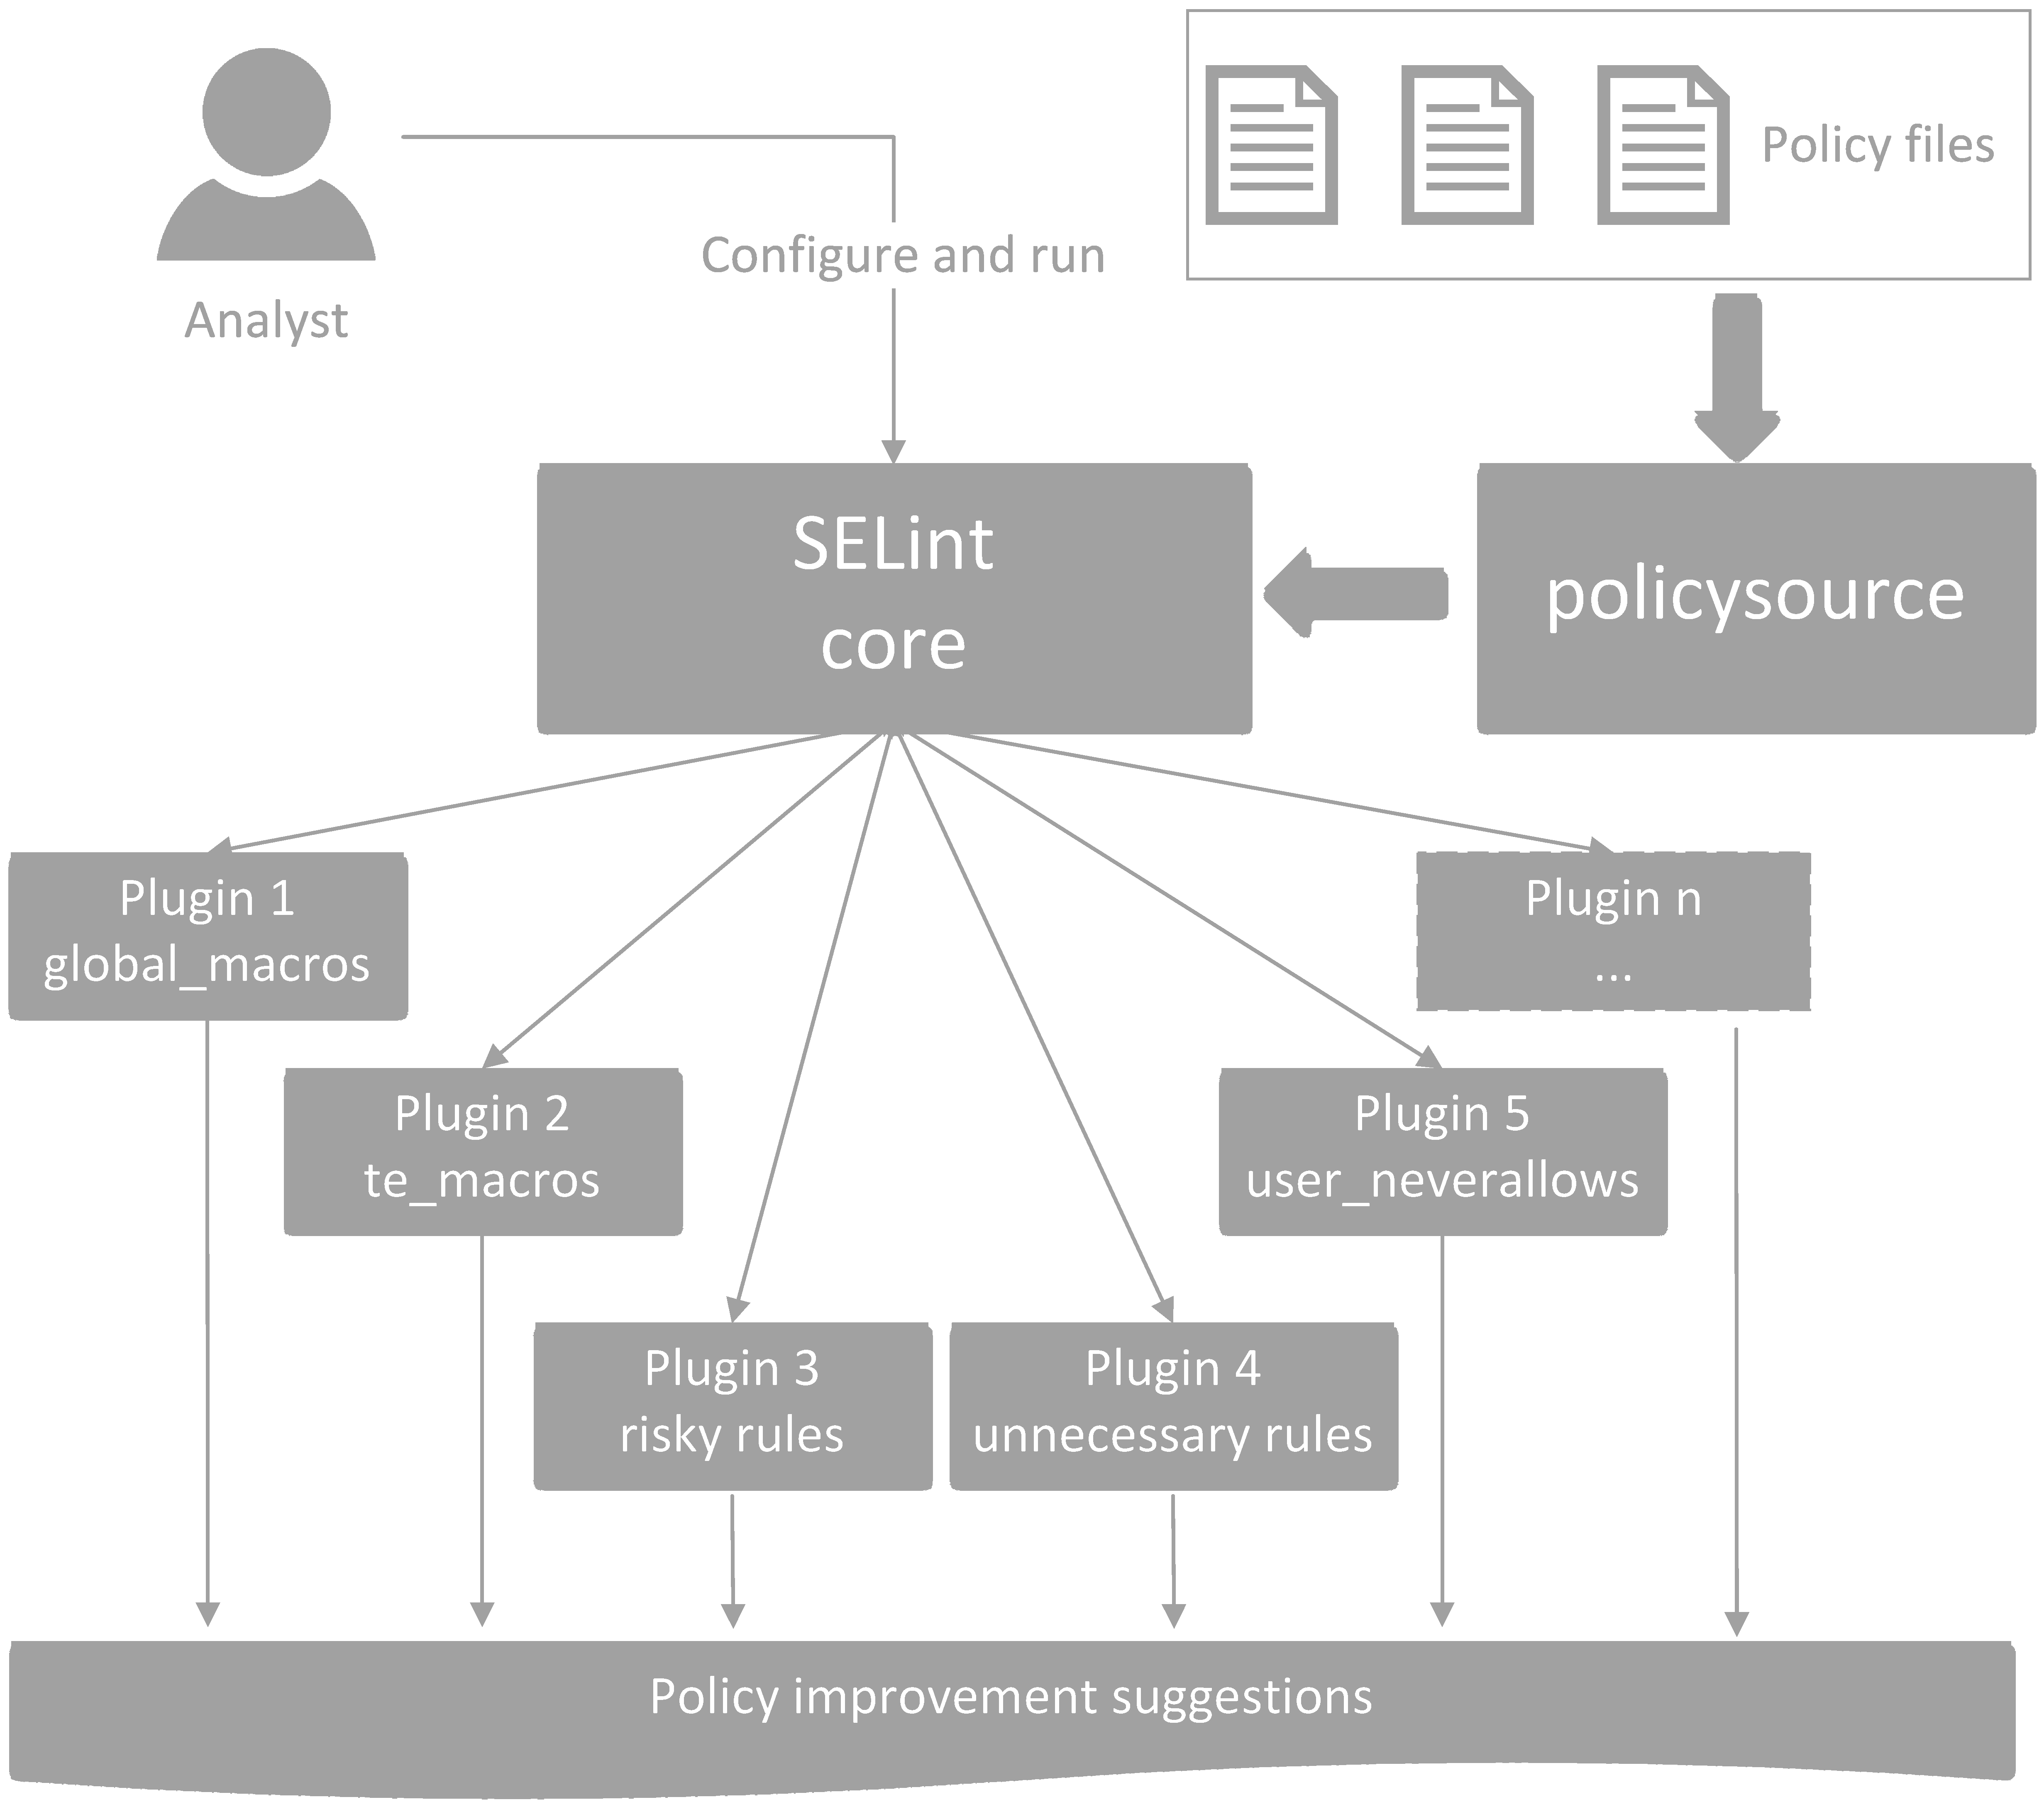
\includegraphics[width=0.80\textwidth]{figures/selint.png}
	\caption{The architecture of SELint (Adapted from Publication III)}
	\label{fig:selint}
\end{figure}

As a result of the above study, Publication II proposes a set of tools that should help both OEMs and security researchers to develop better SEAndroid policies without the above-mentioned pitfalls, including various policy analyzers and virtualization tools. It also implements one such tool, a live SEAndroid policy analyzer (SEAL), that allows performing different policy queries, not only based on the actual policy loaded on a device, but also also based on the run-time device state, i.e. running processes and services, filesystem labeling etc. SEAL allows obtaining fast answers to various questions that a SEAndroid policy writer or analyst might have, such as "\textit{What files can a given running process access on a device?}" or "\textit{What processes can access a given object?}". This significantly simplifies debugging, troubleshooting and studying the given SEAndroid policy and gives a fast way to discover the inconsistencies. 

Publication III presents the design and implementation of a more comprehensive SEAndroid tool, SELint, that provides a framework that can be used to improve SEAndroid policy development. It operates on the SEAndroid policy sources and allows smooth integration into the OEM policy development workflow. The architecture of SELint is shown in Figure~\ref{fig:selint}. It is composed from a SELint core, responsible for the heavy processing of input SEAndroid policy files, and an initial set of SELint plugins that operate on a policy representation provided by the core and able to do the policy analysis. The set of plugins is designed to be extensible and adapt to the needs of different OEMs or security researchers. The initial set of plugins includes: two plugins (\setype{global\_macros} and \setype{te\_macros}) verifying correctness of usage of different types of SEAndroid policy macros, a \setype{user\_neverallows} plugin that allows an OEM-specific verification of additional neverallow rules, an \setype{unnecessary\_rules} plugin that attempts to detect various ineffective rules\footnote{Some rules in SEAndroid policy are only effective in combination with others, such as domain transition rules when a process wants to transition its domain to a different one upon opening a certain type of object.} or rules used for debug purposes, and finally a \setype{risky\_rules} plugin that can be used to categorize SEAndroid access control domains into a set of related ones (untrusted, security-sensitive, core etc.) and display various risk and trust relationships between them in a given policy. For example, it is possible to highlight the access control rules where the access to a security-sensitive object is given to a subject belonging to an untrusted domain.


\section{Application and process isolation using OS-level virtualization}
\label{sec:os-virt}

While traditional access control mechanisms and systems aiming for application and process isolation have existed for decades, recent years have seen the rise of an alternative approach, \textit{OS-level virtualization techniques}, widely known as "\textit{containers}". While originally developed purely to support various virtualization-based use cases, such as server consolidation or application and resource state management, they later on turned into various security-driven use cases, such as application isolation and the Bring Your Own Device (BYOD) scenario\footnote{A single physical device is used for both business and personal purposes that requires a strict isolation between these two environments and limited sharing.}. These additional focus areas brought new security requirements with respect to application and process isolation for OS-level virtualization techniques.

In contrast to the traditional virtualization solutions, like the well-known Xen hypervisor~\cite{xenproject} or Linux Kernel Virtual Machine (KVM)~\cite{kvmproject}, OS-level virtualization only virtualizes the OS kernel resources available to userspace, as opposed to the actual physical hardware resources, and therefore allows processes to share the same host OS kernel. This greatly reduces the performance overhead incurred by the OS-level virtualization and it consequently becomes possible to use this technology for efficient isolation of stand-alone applications or their sets. Despite its popularity, there is a constant debate about the security level that such virtualization provides in practice, as well as attempts to find the gaps in the current implementation. 


\begin{figure}[t]
\centering
\begin{subfigure}{.5\textwidth}
  \centering
  \includegraphics[width=0.8\linewidth]{figures/os-virtualization-sys-model.png}
  \caption{System model}
  \label{fig:osv-1}
\end{subfigure}%
\begin{subfigure}{.5\textwidth}
  \centering
  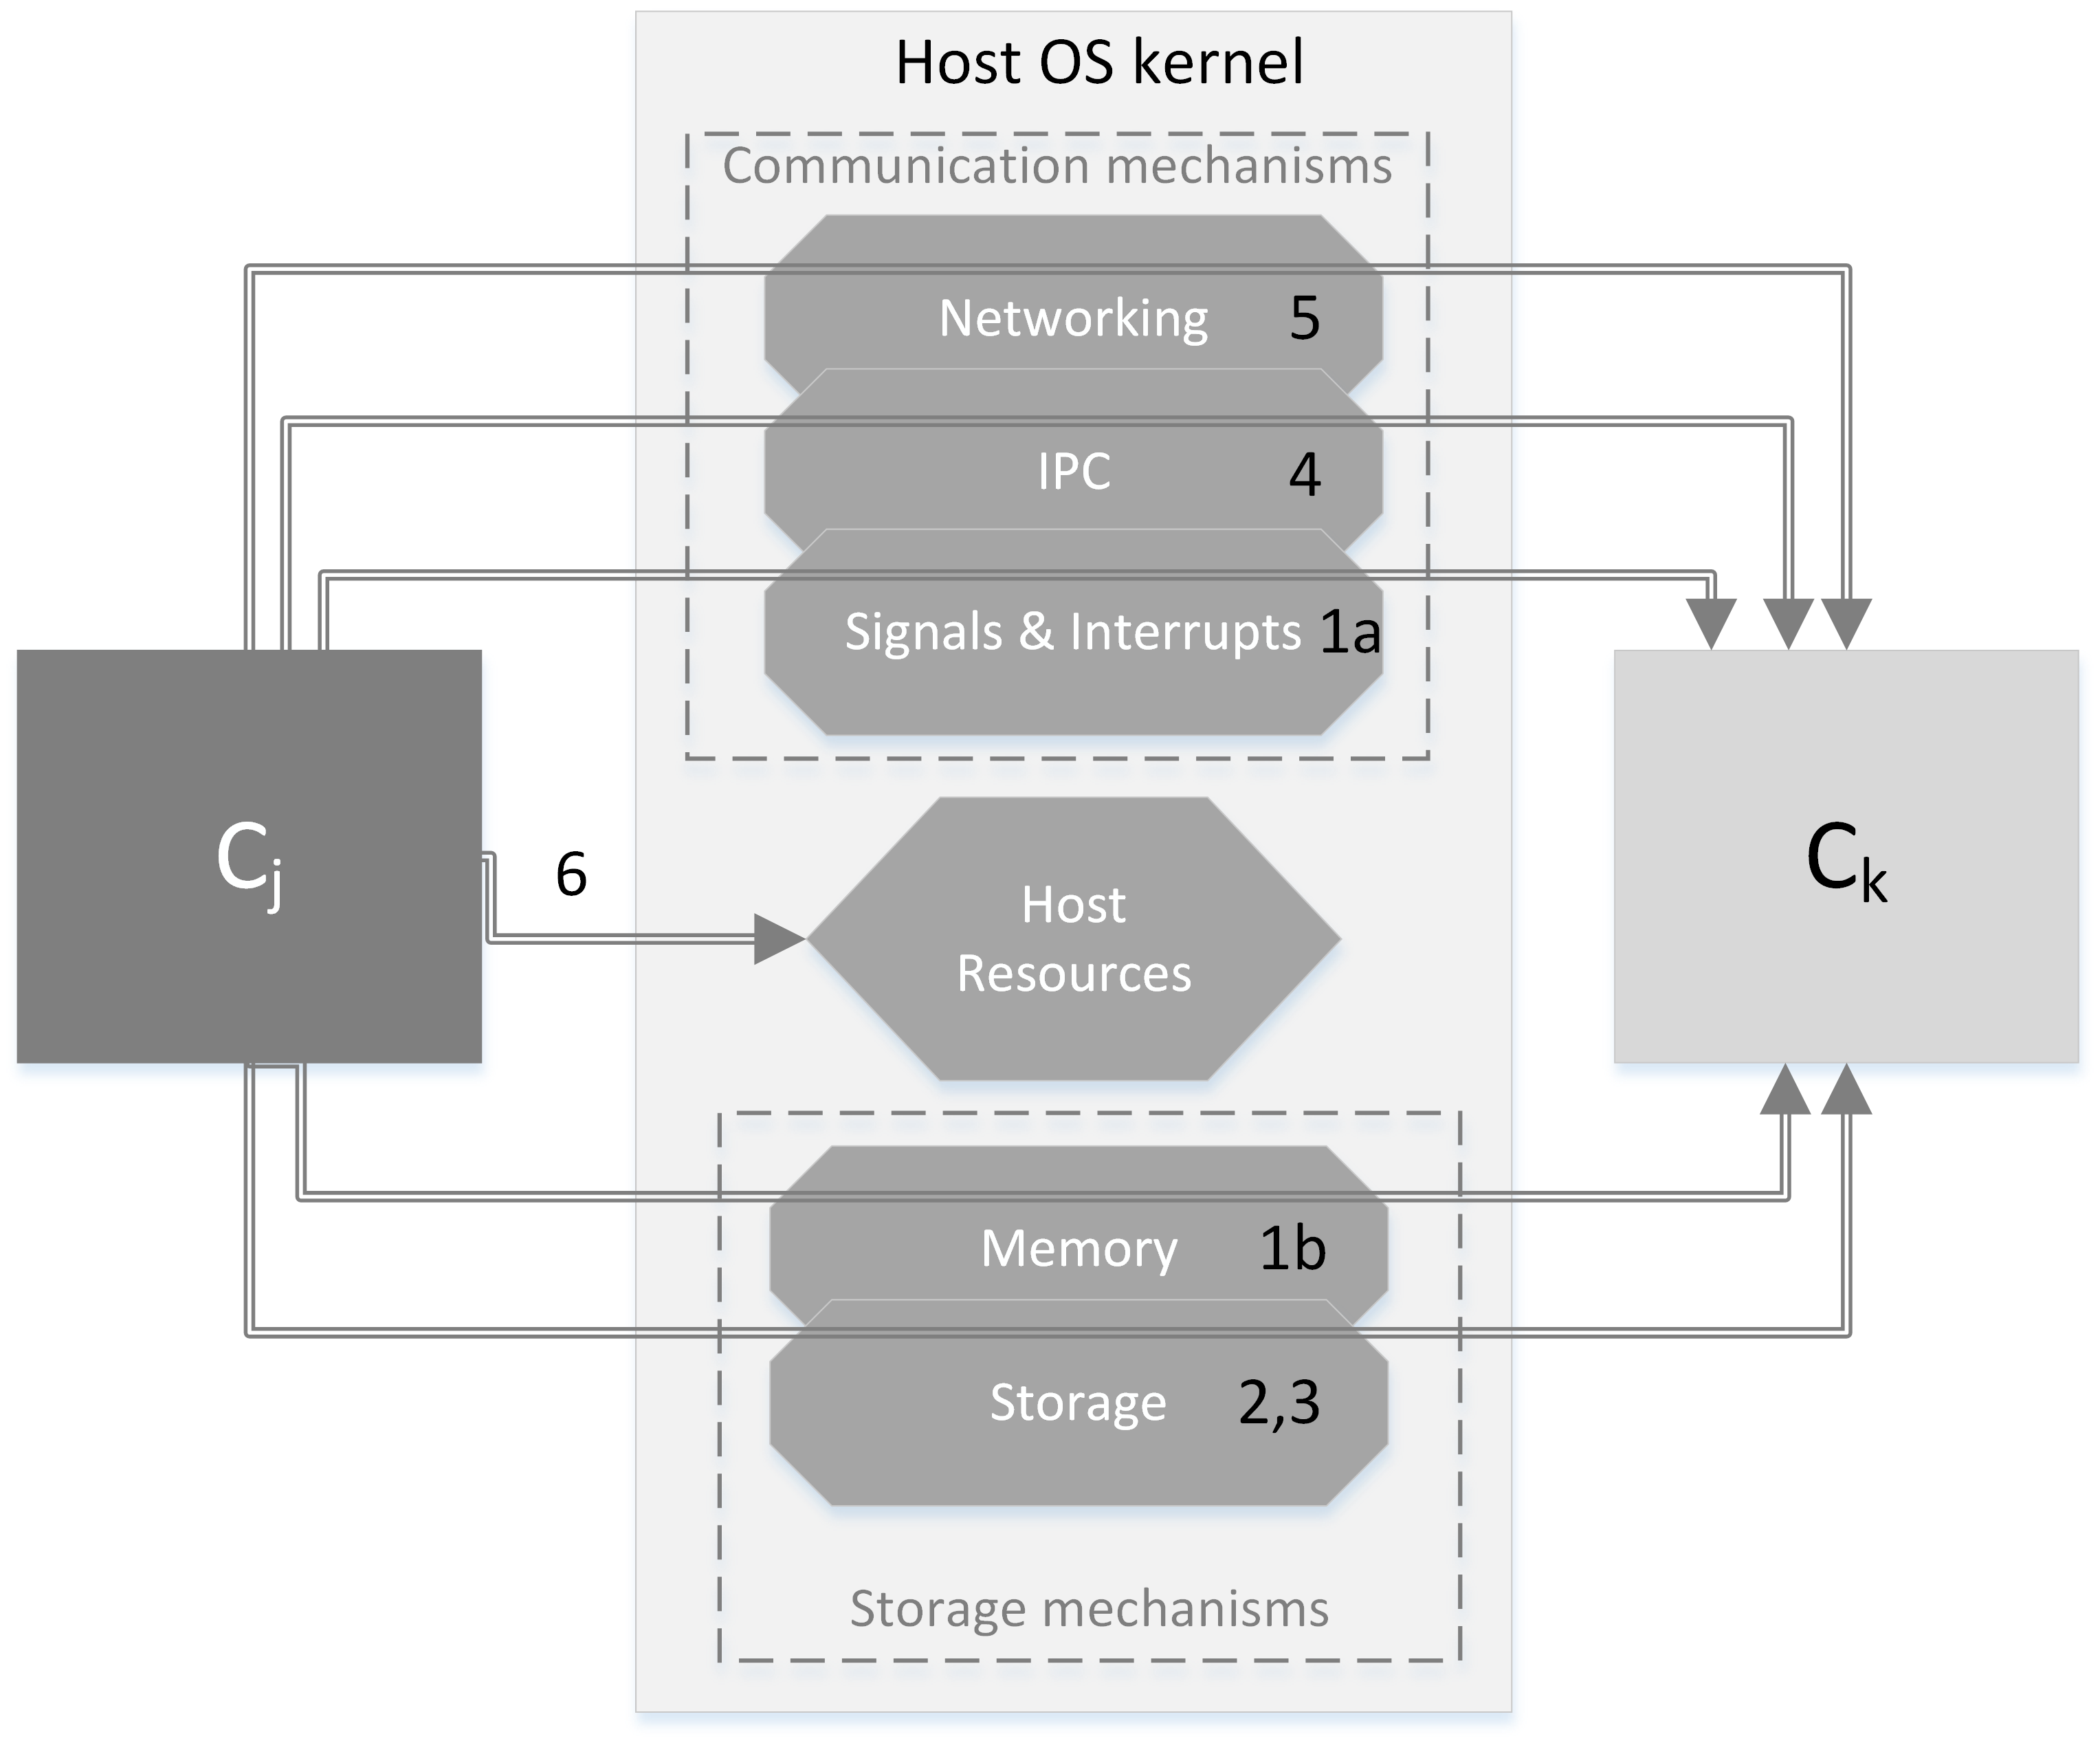
\includegraphics[width=1\linewidth]{figures/OS-virtualization-attacker-model.png}
  \caption{Attacker model}
  \label{fig:osv-2}
\end{subfigure}
\caption{OS-level virtualization. (Adapted from Publication IV)}
\label{fig:os-virtualization}
\end{figure}

Publication IV of this dissertation identifies the security requirements and generic model for a typical OS-level virtualization setup.
The system model for OS-level virtualization is shown in Figure~\ref{fig:osv-1}. The set of containers \setype{C\scriptsize{1}\normalsize..C\scriptsize{N}} is running on top of a shared host OS kernel and a userspace layer. The latter one can be either a minimal layer, only responsible for doing the setup of containers, or a full-fledged host OS userspace layer. The attacker model, shown in Figure~\ref{fig:osv-2}, assumes that an adversary has full control over a certain subset of containers (\setype{C\scriptsize{j}} in Figure~\ref{fig:osv-2}) and attempts to attack either another subset of legitimate containers (\setype{C\scriptsize{k}} in Figure~\ref{fig:osv-2}) running on the same host or the host OS itself. An attacker aims to achieve one of the following end goals: privilege escalation, legitimate container or host compromise or denial-of-service. This can be done by one of the attack groups 1 to 6 shown in Figure~\ref{fig:osv-2}, classified based on typical interfaces available to a UNIX-compliant OS. These attack groups are then converted into security requirements that each OS-level virtualization solution must fulfill in order to provide strong isolation guarantees: separation of processes, filesystem isolation, device isolation, IPC isolation, network isolation and resource management.   

Publication IV analyzes 6 different OS-level virtualization solutions against the above security requirements and outlines the differences in the provided level of isolation. It also summaries the state of OS-level virtualization in the mainline Linux kernel, implemented using "\textit{kernel namespaces}"~\cite{biederman2006}. A kernel namespace is a set of identifiers representing the global kernel resources, such as process and user ids, filesystem mounts, network interfaces, IPC objects, etc. A \textit{container} in the mainline Linux kernel is therefore a collection of such kernel namespaces that restrict visibility and communication between processes running in different kernel namespaces. In addition, Publication IV also defines a number of gaps that were limiting the usage of this technology in environments with strict security isolation requirements: the need for security namespaces, a better support for resource management, etc. In recent years, some of these gaps have progressed towards robust solutions and many new ones have been identified. Below is a summary of recent changes to the mainline Linux kernel in the relevant areas that help improve the OS-level virtualization in the mainline Linux kernel:  

\begin{itemize}
	\item \textbf{Security (LSM) namespaces.} Publication IV outlines the importance of having security namespaces implemented in order to be able to enforce independent mandatory access control security policies for different containers, as well as for the host OS. In recent years, this topic has received significant attention from the Linux kernel security community, with a number of mainstream Linux Security Modules (LSMs), such as Smack~\cite{smack} and AppArmor~\cite{bauer2006paranoid}, proposing their approaches and implementations~\cite{smackns},~\cite{apparmorns}. Unfortunately, these implementations are currently LSM-specific and only allow the creation of independent container-specific policies within the same LSM. However, this is a significant step forward and discussions on a unified solution continue.
	\item \textbf{Cgroups namespaces.} Cgroups kernel subsystem~\cite{cgroupsv2}, that is actively used in the mainline Linux kernel to implement resource management, underwent a major change at the end of 2015 in an attempt to address various gaps and criticism from its users~\cite{rosen2016}. The new solution, cgroups v2~\cite{cgroupsv2}, added many new features, including namespace support for cgroups themselves. The latter allows having independent cgroups hierarchies for different containers and restricts each container to only view its own cgroups rules. 
	\item \textbf{Automatic loading restriction support.} A process running inside a malicious container might try to use kernel features like automatic module loading as a way to escape the container. It can be done by requesting a kernel feature that is provided by a module that is not loaded in the kernel. In order to satisfy the request, the kernel would automatically load the module, despite the process having no permissions to ask about such an operation explicitly. In turn, this module can be potentially an old and vulnerable one, exposing the host OS kernel to easy attacks. A recent proposal~\cite{harouni2017} to address this issue and create suitable controls has been discussed in the mainline Linux kernel community, and while the implementation details will still likely change, it is considered as an important security improvement. 
  \item \textbf{Keyring namespace support.} The mainline Linux kernel has a convenient facility, Kernel Keyring~\cite{keyrings}, for in-kernel storage and management of security keys and authentication tokens. The keys stored in these \textit{keyrings} are available not only for usage within the kernel itself, but also for userspace processes. From a security point of view, different containers and the host OS should naturally have separated kernel keyrings, but this hasn't yet been implemented in the mainline Linux kernel. Similar to other cases, an initial proposal~\cite{howells2016} by the keyring subsystem maintainer that separates keyrings between different user namespaces has been discussed by the Linux kernel security community and remains the expected future direction. 
	\item \textbf{IMA policy namespaces.} In addition to MAC mechanisms provided by various LSMs, the mainline Linux kernel has an Integrity Measurement Architecture (IMA)~\cite{ima} subsystem that aims to detect if files have been accidentally or maliciously modified when the device is in the offline state. This is done by calculating a reference hash value over the file content and attributes and comparing it to the newly calculated value every time the file is accessed. Similarly as for LSMs, IMA operates on a policy that defines what files should be measured and when, as well as various exceptions. OS-level virtualization brings a similar requirement to IMA as for LSMs: the IMA policy needs to be namespaced in order to be able to have separate independent policies for the host OS and different containers. Active discussions on the best direction for IMA policy namespacing continue in the Linux kernel security community as well as first implementation proposals have been presented~\cite{magalhaes2017}. 
	\item \textbf{Stricter handling of POSIX capabilities.} A very recent proposal~\cite{Bandewar2017} introduces a mechanism to limit the usage of POSIX capabilities~\cite{caps} inside user namespaces. This can be a very desired feature for further security hardening for OS-level virtualization since it is currently possible for a process that entered a user namespace to acquire a wide range of POSIX capabilities within this namespace and try to misuse them. 
\end{itemize}


\section{Discussion}

OS-level virtualization methods have gained a lot of attention and interest in the Linux community due to their usability aspects. It is much easier to spawn a set of separate containers with independently running applications than achieving the same setup using MAC mechanisms. However, if sharing of data or IPC communication between these applications is required, then the setup quickly gets more complicated. Therefore our answer to the \textbf{\textit{security of OS-level virtualization}} research question is the following. While the implementation of the OS-level virtualization in the mainline Linux kernel continues to evolve and improve, the classical mandatory access control schemes are still required to be jointly used in order to provide the highest possible level of isolation, support fine-grained access control policies and minimize the security risks. Security architects must understand the details and the limitations of OS-level virtualization in order to make well-grounded choices on a set of isolation mechanisms for their systems in order to fulfill given security requirements. Publication IV of this dissertation presents a good model for such evaluation and comparison of available mechanisms, as well as guidance on identifying the missing isolation gaps. 

The SEAndroid MAC continues to be the main access control enforcement point of Android OS with all major OEMs now accustomed to the task of working with SEAndroid policies. The evaluation of initial SEAndroid policies, in Publication II, has answered the \textit{\textbf{access control deployment challenges}} research question by summarizing the main challenges and pitfalls of SEAndroid policy development and deployment. Publication II has also been crossed-referenced in the official Google SEAndroid documentation~\cite{seanroidsize}. Following the \textbf{\textit{practical tools for access control development and deployment}} research question, Publications II and III propose the SEAndroid tools, SEAL and SELint. These tools are being used by the Android community with numerous private forks on the project code trees and bug reports by the users once in a while\footnote{https://github.com/seandroid-analytics}. The SELint tool fulfills the set of its main functional R1 - R4 requirements defined in Section IV of Publication III by exhibiting an acceptable performance overhead, allowing its usage by ordinary users (after an initial expert configuration), being flexible and easy extensible. Due to the nature of SELint, i.e. the tool targets OEMs and internal use within their systems, it is hard to make an estimate on its usage in the real world, but a detailed evaluation of the tool can be found in Section V of Publication III. 

